%!TEX root = ../doc.tex
\chapter{Konzept}
\label{sec:konzept}
Aus den Anforderungen ist klar ersichtlich, dass eine eigene Benutzeroberfläche entwickelt werden soll, die über die Programmierschnittstelle von LoBo kommunizieren soll. Die nicht funktionelle Anforderung NFREQ-001 verlangt eine Web Browser-kompatible Benutzeroberfläche und disqualifiziert eine zu installierende Desktop Client Anwendung. Trotz der Limitierung der Lösungsmöglichkeiten bleiben bei der Entwicklung einer Benutzeroberfläche im Web viele Fragen offen. Im Folgenden werden die Technologie- sowie Architekturentscheidungen vorgestellt und begründet.

\section{Web Modell}
Traditionelle Websites bestehen aus mehreren \textit{Hyper Text Markup Language} (HTML) Seiten und liefern diese, wenn der Client sie anfordert, aus. Es gibt verschiedene Programmiersprachen, die es erlauben zum Zeitpunkt des Aufrufs den Code, der in diesen HTML Seiten vorhanden ist, zu interpretieren und das entsprechende Resultat auszuliefern. \textit{PHP Hypertext Preprocessor}\footnote{Offizielle Website von PHP: \url{http://php.net/}} (PHP) ist eine der bekanntesten Programmiersprachen. Aber auch Python bietet mit dem Framework \textit{Django}\footnote{Offizielle Website von Django: \url{https://www.djangoproject.com}} eine ähnliche Funktionalität. Mit der zunehmende Möglichkeiten im Web sowie der immer grösseren Komplexität wurden andere Modelle für das Web entwickelt. Mit der offiziellen Spezifikation des \textit{XMLHttpRequest Object} am 5. April 2006 \citep[]{w3cXMLHttpRequest} und dessen Einsatz von Google in Webapplikationen wie Gmail und Google Maps wurde die Entwicklung von \textit{Single-page application} (SPA) ermöglicht. Mit \textit{XMLHttpRequest} ist es möglich nach dem Laden der Website eine Anfrage an den Server zu schicken ohne dabei die gesamte HTML Seite neu zu laden. Für die Ausführung dieser \textit{XMLHttpRequest} Anfragen wird eine clientseitige Skriptsprache benötigt. Trotz vereinzelten Alternativen ist JavaScript der Standard bei den browserfähigen clientseitigen Skriptsprachen. Dies ist mitunter auch ein Grund warum SPA Webseiten mit JavaScript erstellt werden. In den Abbildungen  \ref{fig:requestHtml} und \ref{fig:requestXHtml} \footnote{Bilder von \url{https://blog.4psa.com/an-intro-into-single-page-applications-spa/}} ist der Unterschied zwischen einer konventionellen Website und einer SPA veranschaulicht.

\begin{figure}[ht]
	\centering
  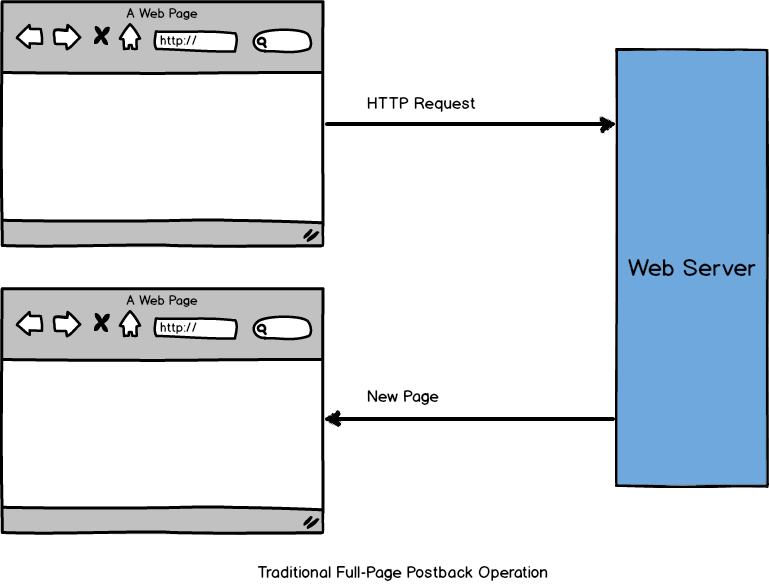
\includegraphics[width=0.88\textwidth]{images/requestHtml.png}
	\caption{Visualisierung einer Anfrage in einer konventionellen Webseite}
	\label{fig:requestHtml}
\end{figure}

\begin{figure}[ht]
	\centering
  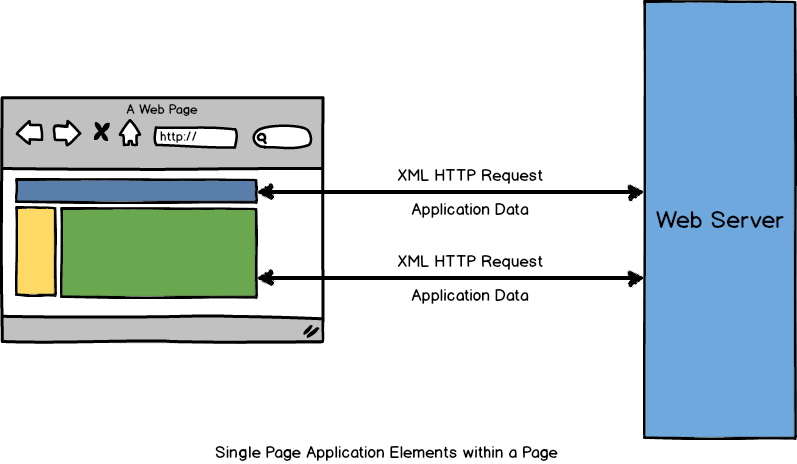
\includegraphics[width=0.88\textwidth]{images/requestXHtml.png}
	\caption{Visualisierung einer Anfrage in einer Single-page Applikation}
	\label{fig:requestXHtml}
\end{figure}


\subsection{Single-page application}
\textit{Single-page application} (SPA) haben viele Vorteile gegenüber traditionellen Webseiten. Die gesamte Webseite kann mit wenigen Anfragen an den Server geladen werden. Im Wesentlichen werden nur drei Anfragen (1. HTML Seite, 2. Cascading Style Sheets (CSS), 3. JavaScript) benötigt. Alle weiteren Daten wie z.B. Benutzerdaten aus der Datenbank werden asynchron mit einer \textit{XMLHttpRequest} Anfrage, während die Webseite im Browser aufgebaut wird, geladen. Dies hat den Vorteil, dass die Webseite bedeutend schneller geladen wird und trägt damit zur Benutzerfreundlichkeit bei. Im Folgende ist eine nicht abgeschlossene Liste mit den Vorteilen von SPA.
\begin{description}
	\item[Entlastung] Die Benutzeroberfläche wird komplett im Browser erstellt und benötigt dafür keine Ressourcen vom Server.
	\item[Entkopplung] Daten und Businesslogik sind nicht mehr an die Visuellen Elemente gebunden.
	\item[Performant] Single-page Applikationen verwalten ihren eigenen Status und benötigten dafür weniger Informationen vom Server.
\end{description}
SPA setzten voraus, dass der Server eine definierte Schnittstelle besitzt, über welche Daten geladen bzw. geschrieben werden können. Dies hat zusätzlich den Vorteil, dass auch Applikationen anderer Plattformen wie z.B. Android oder iOS auf diese Schnittstellen zugreifen können.
\newline{}
Ein grosser Nachteil von Single-Page Applikationen ist die Lesbarkeit des auszuführenden Codes. JavaScript ist eine Skriptsprache, dir zur Laufzeit interpretiert und ausgeführt wird. Dies bedeutet dass der gesamte Code im Browser vorhanden ist und für den Benutzer lesbar ist. Es gibt Werkzeuge, die versuchen diesen Code unleserlich zu machen indem Variablen umbenennt und Leerzeichen entfernt werden, aber mit Energie und Geduld kann auch dies wieder lesbar gemacht werden.

\subsection{Mini-Backend}
Für die Auslieferung der \textit{Single-page application} wird nur ein Webserver wie z.B. Apache\footnote{Apache ist ein weitverbreiteter opensource Webserver \url{https://httpd.apache.org/}} oder Nginx benötigt. Die SPA kann aber auch von einem Webserver ausgeliefert werden, welcher eigene Logik besitzt. Im Rahmen dieser Bachelorarbeit nenne ich die Benutzung eines Webservers mit eigener Logik Mini-Backend. Es existieren mehrere Plattformen in verschiedenen Programmiersprachen, mit welchen die Entwicklung eines Mini-Backend möglich wäre.  Node.js\footnote{Node.js ist eine Serverseitige Plattform \url{https://nodejs.org}} ist eine serverseitige Plattform welche auf JavaScript basiert und die Möglichkeit bietet, Webseiten auszuliefern und eigene Logik auszuführen. Diese Logik bzw. dieser Code befindet sich immer auf dem Server und kann von den Benutzer nicht gelesen werden. Node.js kann die gesamte Businesslogik eines Projektes beinhalten oder aber nur Webanfragen weiterleiten.

\subsection{Fazit}
Obwohl die Logik für die zu entwickelnde Benutzeroberfläche ausschliesslich in der SPA ausgeführt werden könnte, hat der Einsatz eines sogenannten Mini Backends erhebliche Vorteile. LoBo benutzt für die Authentifizierung einen Schlüssel, mit welchem alle Anfragen \textit{gehasht} werden müssen. Der entstandene Hash wird im Header jeder Anfrage mitgeschickt. Dadurch kann LoBo die Authenzität und Integrität der Anfragen sicher stellen. Dieses hashing könnte in der SPA geschehen, hat jedoch den Nachteil, dass der Schlüssel von den Benutzer ausgelesen werden kann. Zusätzlich vereinfacht der Einsatz eines Mini-Backend die Skalierung. Weil die Mini-Backends nicht auf eine Datenbank zugreifen, können einfach mehrere Instanzen gestartet werden und ein zusätzlicher Webserver verteilt die Anfragen auf die verfügbaren Instanzen. Die Mini-Backends können auch mit verschiedenen LoBo Systemen kommunizieren. Dies verhindert einen Flaschenhals bei einem Anstieg der Benutzerzahlen. Im Rahmen dieser Bachelorarbeit wird eine Single-page Applikation mit JavaScript entwickelt und ein Mini-Backend welches auf Node.js basiert. Node.js wurde ausgewählt, weil es in der gleichen Sprache programmiert wird wie die SPA und dadurch einige Vorteile für den Entwickler bietet. Der Entwickler braucht während der Entwicklung nicht den Kontext zu wechseln und kann unter Umständen die gleichen Ressourcen für die SPA wie auch das Mini-Backend verwenden.

\section{JavaScript}
JavaScript ist eine zurzeit populäre Programmiersprache, die zu einem grossen Teil für dynamischen Aspekte einer Webseite verantwortlich ist, aber auch Serverseitig zum Einsatz kommt. Obwohl während den Anfängen von JavaScript mehrere Interpretationen der Sprache existierten, ist JavaScript heute der einzige Dialekt welcher auf der EcmaScript Spezifikation basiert und interpretiert wird. JavaScript wird von allen grossen Browsern mit ihren jeweiligen Implementationen unterstützt. Im Folgenden eine Liste der JavaScript Engines der bekanntesten Browsers\footnote{Liste von Wikipedia \url{https://en.wikipedia.org/wiki/ECMAScript}}.
\begin{description}
	\item[SpiderMonkey] wird von Mozilla für den Browser Firefox entwickelt.
	\item[V8] wird von Google für den Browser Chrome entwickelt.
	\item[JavaScriptCore] wird von Apple für den Browser Safari entwickelt.
	\item[Chakra] wird von Microsoft für den Browser Edge entwickelt.
\end{description}
V8 von Google wird unter anderem auch für Node.js verwendet, welches im Rahmen dieser Bachelorarbeit für das Mini-Backend verwendet wird.

\subsection{ES2015}
Die Sprache hat im Juni 2015 eine lang erwartet neue Version bekommen. Ecma International\footnote{European Computer Manufacturers Association \url{http://www.ecma-international.org/}} welche die Spezifikationen für die Programmiersprache JavaScript schrieb, hat die Version EcmaScript 2015 veröffentlicht und damit der Sprache einige neue Funktionen verliehen. Mit EcmaScript 2015 (ES2015) können Klassen erstellt werden und mit einem Module System Klassen, Objekte, Funktionen und Variablen exportiert wie auch importiert werden. Dank dieser Erneuerung ist es bedeutend einfacher JavaScript Code zu unterhalten und zu pflegen. Er kann in verschiedene Module unterteilt werden und ist dadurch auch besser lesbar. Einige der Erneuerungen machen auch Helfer Bibliotheken wie \textit{underscore.js} oder \textit{jquery} überflüssig, was wiederum zur Leistung beiträgt.

\subsection{Backend Framework}
Für Node.js existieren mehrere Webserver Frameworks, die für den Einsatz im Rahmen dieser Bachelorarbeit eingesetzt werden können. 3 populäre Frameworks sind Express.js\footnote{Web Framework für Node.js \url{http://expressjs.com/}}, Koa.js\footnote{Web Frameork für Node.js \url{http://koajs.com/}} und hapi.js\footnote{Web Framework für Node.js \url{http://hapijs.com/}}. Jedoch Express.js ist das populärste Framework und findet auf Github die grösste Unterstützung.\citep[]{nodejsframeworks}. Die Entwicklung der Mini-Backends benötigt keine aussergewöhnlichen Anforderungen und hat mit Express.js alle Ansprüche abgedeckt.

\subsection{Frontend Framework}
In JavaScript existieren unzählige Frameworks, die etliche Anwendungsfälle unterstützen. Obwohl eine Single-Page Applikation auch ohne Framework und Helfer-Bibliothek entwickelt werden kann, können Frameworks zur Stabilität und zum Erfolg der Webseite beitragen. Frameworks wie Angular\footnote{Javascript Framework von Google \url{https://angularjs.org/}} und Ember.js\footnote{Javascript Framework aus der OpenSource Gemeinschaft \url{http://emberjs.com/}} unterstützen die Entwicklung einer \textit{Model View Controller} (MVC) SPA erheblich. Angular stellt z.B. einen Service (\textit{\$resource}) zur Verfügung, mit welchem alle \textit{XMLHttpRequest}-Anfragen ausgeführt werden können. Die Handhabung im Falle eines Fehlers kann zentral implementiert werden und auch die Transformation von empfangenen sowie zu versendenden Daten kann mit dem Service verwaltet werden. In Ember.js wird eine Datenverwaltungs-Komponente zur Verfügung gestellt, die die gesamte Synchronisation der Daten mit einem Backend übernimmt. Sofern das Backend eine standardisierte JSON REST\footnote{REST steht für \textit{Representational State Transfer} und bezeichnet ein Programmierparadigma} Programmierschnittstelle besitzt, kann diese Synchronisation, die Daten erstellt, bearbeitet, lädt und löscht, mit wenigen Zeilen Code implementiert werden. Diese Beispiele sind nur vereinzelte Einblicke in die Möglichkeiten der Frameworks. Frameworks bringen aber auch Nachteile mit sich. Sobald ein Anwendungsfall implementiert werden soll, der nicht dem Framework entspricht, kann es kompliziert und fehleranfällig werden.
\newline{}
Ein relativ neues JavaScript Framework ist \textit{React}\footnote{JavaScript Framework von Facebook \url{https://facebook.github.io/react/}}, welches von Facebook entwickelt wird. React setzt im Gegensatz zu MVC Frameworks eine andere Philosophie um. Zum einen wird in React mit Komponenten, die wiederum Subkomponenten beinhalten, gearbeitet. Zum anderen wird das Programmierparadigma \textit{Data Down, Actions up} umgesetzt. In diesem Programmierparadigma wird den Komponenten die benötigten Daten übergeben und die Komponenten rufen eine Methode auf, die die bearbeiteten Daten zurück gibt. Zusätzlich werden die \textit{Templates}, die für die visuelle Repräsentation der Komponenten benötigt werden nicht wie üblich in HTML geschrieben sondern in JSX\footnote{JSX steht für \textit{JavaScript Syntax extension} und erlaubt das Schreiben von HTML in JavaScript}, womit der gesamte Code einer Komponente in der gleichen Datei geschrieben werden kann. Auch von Facebook stammt die Applikations Architektur \textit{Flux}. \textit{Flux} besteht aus hauptsächlich aus einem \textit{Dispatcher}, \textit{Store} und den \textit{Views} und baut auf einigen wenigen Prinzipien auf, die in der folgenden Liste erklärt werden.
\begin{description}
	\item[Unidirektionaler Datenfluss] Daten fliesen immer in eine Richtung. Jede Änderung der Daten findet über eine Aktion statt.
	\item[Klare Trennung der Kontrolle] Die Kontrolle über die Daten befindet sich in den \textit{Stores} und diese können von Aussen nicht verändert werden.
	\item[Zentralisierter Dispatcher] Es existiert nur ein \textit{Dispatcher}, welcher alle \textit{Stores} über eine neu Aktion informiert. Dadurch wird garantiert, dass immer nur eine Aktion aufs mal ausgeführt wird.
\end{description}
Flux und die Prinzipien sind in der Abbildung \ref{fig:flux} dargestellt.

\begin{figure}[ht]
	\centering
  
\includegraphics[width=0.88\textwidth]{images/flux.png}
	\caption{Darstellung des Programmierparadigma Flux}
	\label{fig:flux}
\end{figure}
Flux und React können kombiniert werden und ergeben dadurch ein stabiles, modernes und fehlerarmes JavaScript Framework.

\subsection{Fazit}
Aus den Anforderungen in Kapitel \ref{sec:anforderungsanalyse} wird klar, dass die gleichen Eingabemasken an verschiedenen Stellen zum Einsatz kommen. Die Eingabe einer Adresse wird in mehreren Anforderungen benötigt. Für diese Anforderung spricht ein Framework wie React, welches diese Eingabemasken als Komponenten einmal implementiert und an verschiedene Stellen zu Verfügung stellt. Auch der Aufbau einer Schritt für Schritt Eingabe lässt sich in Komponenten und Subkomponenten praktisch umsetzen. Weil für die Erstellung eines Auftrags in LoBo einem klaren Prozess gefolgt werden muss, eignet sich der Einsatz von Flux. Mit Flux ist die gesamte Single-page Applikation weniger störungsanfällig und hat zu jedem Zeitpunkt einen klaren Zustand. Im Rahmen dieser Bachelorarbeit wird die zu erstellende Benutzeroberfläche mit React und Flux entwickelt.

\section{Prozess}
Die Erstellung eines Auftrages hat nur zwei Szenarien. Die Start und Zieladresse sind entweder im gleichen Versorgungsgebiet oder befinden sich in unterschiedlichen. Die Single-Page-Applikation weiss dies nicht und es ist Aufgabe des Mini-Backends dies herauszufinden. Davor muss aber zuerst ein Auftrag erstellt werden. Mit dem gewonnen \textit{Tasktoken} werden die verifizierten Adressen als Stops hinzugefügt. Danach wird im Mini-Backend die Methode \textit{compiletask} aufgerufen, welche herausfinden soll, ob und welche Stops hinzugefügt werden sollen. Die Abbildung \ref{fig:compiletask} soll die Aufgabe der Methode grafisch darstellen.

\begin{figure}[ht]
	\centering
  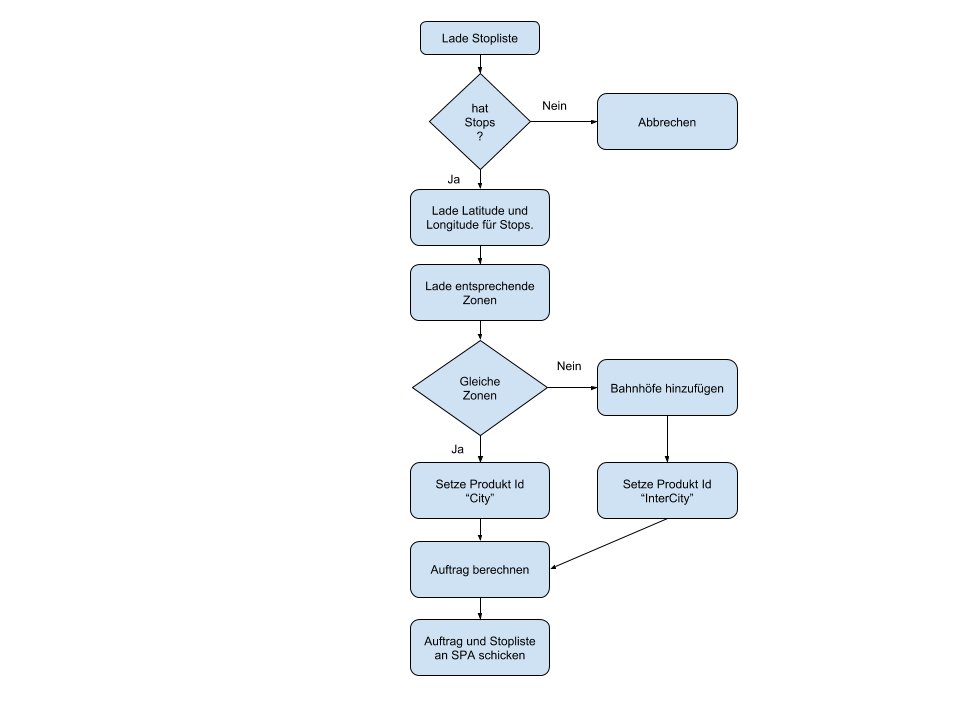
\includegraphics[width=0.88\textwidth]{images/compileTask.png}
	\caption{Darstellung der compileTask Methode}
	\label{fig:compiletask}
\end{figure}

Sollten die Start- und Zieladresse in unterschiedlichen Versorgungsgebieten liegen, werden die verfügbaren Bahnverbindungen angezeigt. Ansonsten werden direkt die Kontaktinformationen für die Start- und Zieladresse gesammelt. Danach wird der Auftrag bestellt und der Benutzer bekommt eine Bestätigung.


\section{Architektur}
\label{sec:architektur}

\subsection{Mini-Backend}
Das Backend hat 2 elementare Aufgaben. Das Ausliefern der SPA und das Bereitstellen der Schnittstelle, mit welcher die SPA kommuniziert. Die SPA befindet sich in einem Verzeichnis und wird bei einem Aufruf direkt ausgeliefert. Alle Anfragen der SPA werden an eine bestimmte URL gesendet, die mit der entsprechenden Antwort oder einem Fehler antwortet. Das Mini-Backend soll aber nicht nur die Anfragen von der SPA an LoBo weiterleiten sondern auch die Komplexität gewisser Prozessabläufe vereinfachen. Obwohl LoBo viele Schnittstellenendpunkte zur Verfügung stellt, werden für gewisse Funktionen mehrere Anfragen benötigt. Für die Abfrage ob eine bestimmte Strassenadresse in einem Gebiet liegt, welches von Imagine Cargo versorgt wird, werden 3 Anfragen an LoBo benötigt. Zuerst muss in LoBo ein neuer Auftrag erstellt werden, mit dem dadurch gewonnen Auftragstoken muss eine Adresse hinzugefügt werden. Zuletzt muss eine Anfrage gestellt werden, die überprüft ob der Auftrag konform ist. Die Fehlermeldung dieser Anfrage bestimmt, ob die Adresse in einem Versorgungsgebiet von ImagineCrago liegt. Der gesamte Ablauf ist in Abbildung \ref{fig:addressverify} grafisch dargestellt. Darin ist zu sehen, wie viel Arbeit vom Mini-Backend gehandhabt wird.

\begin{figure}[ht]
	\centering
  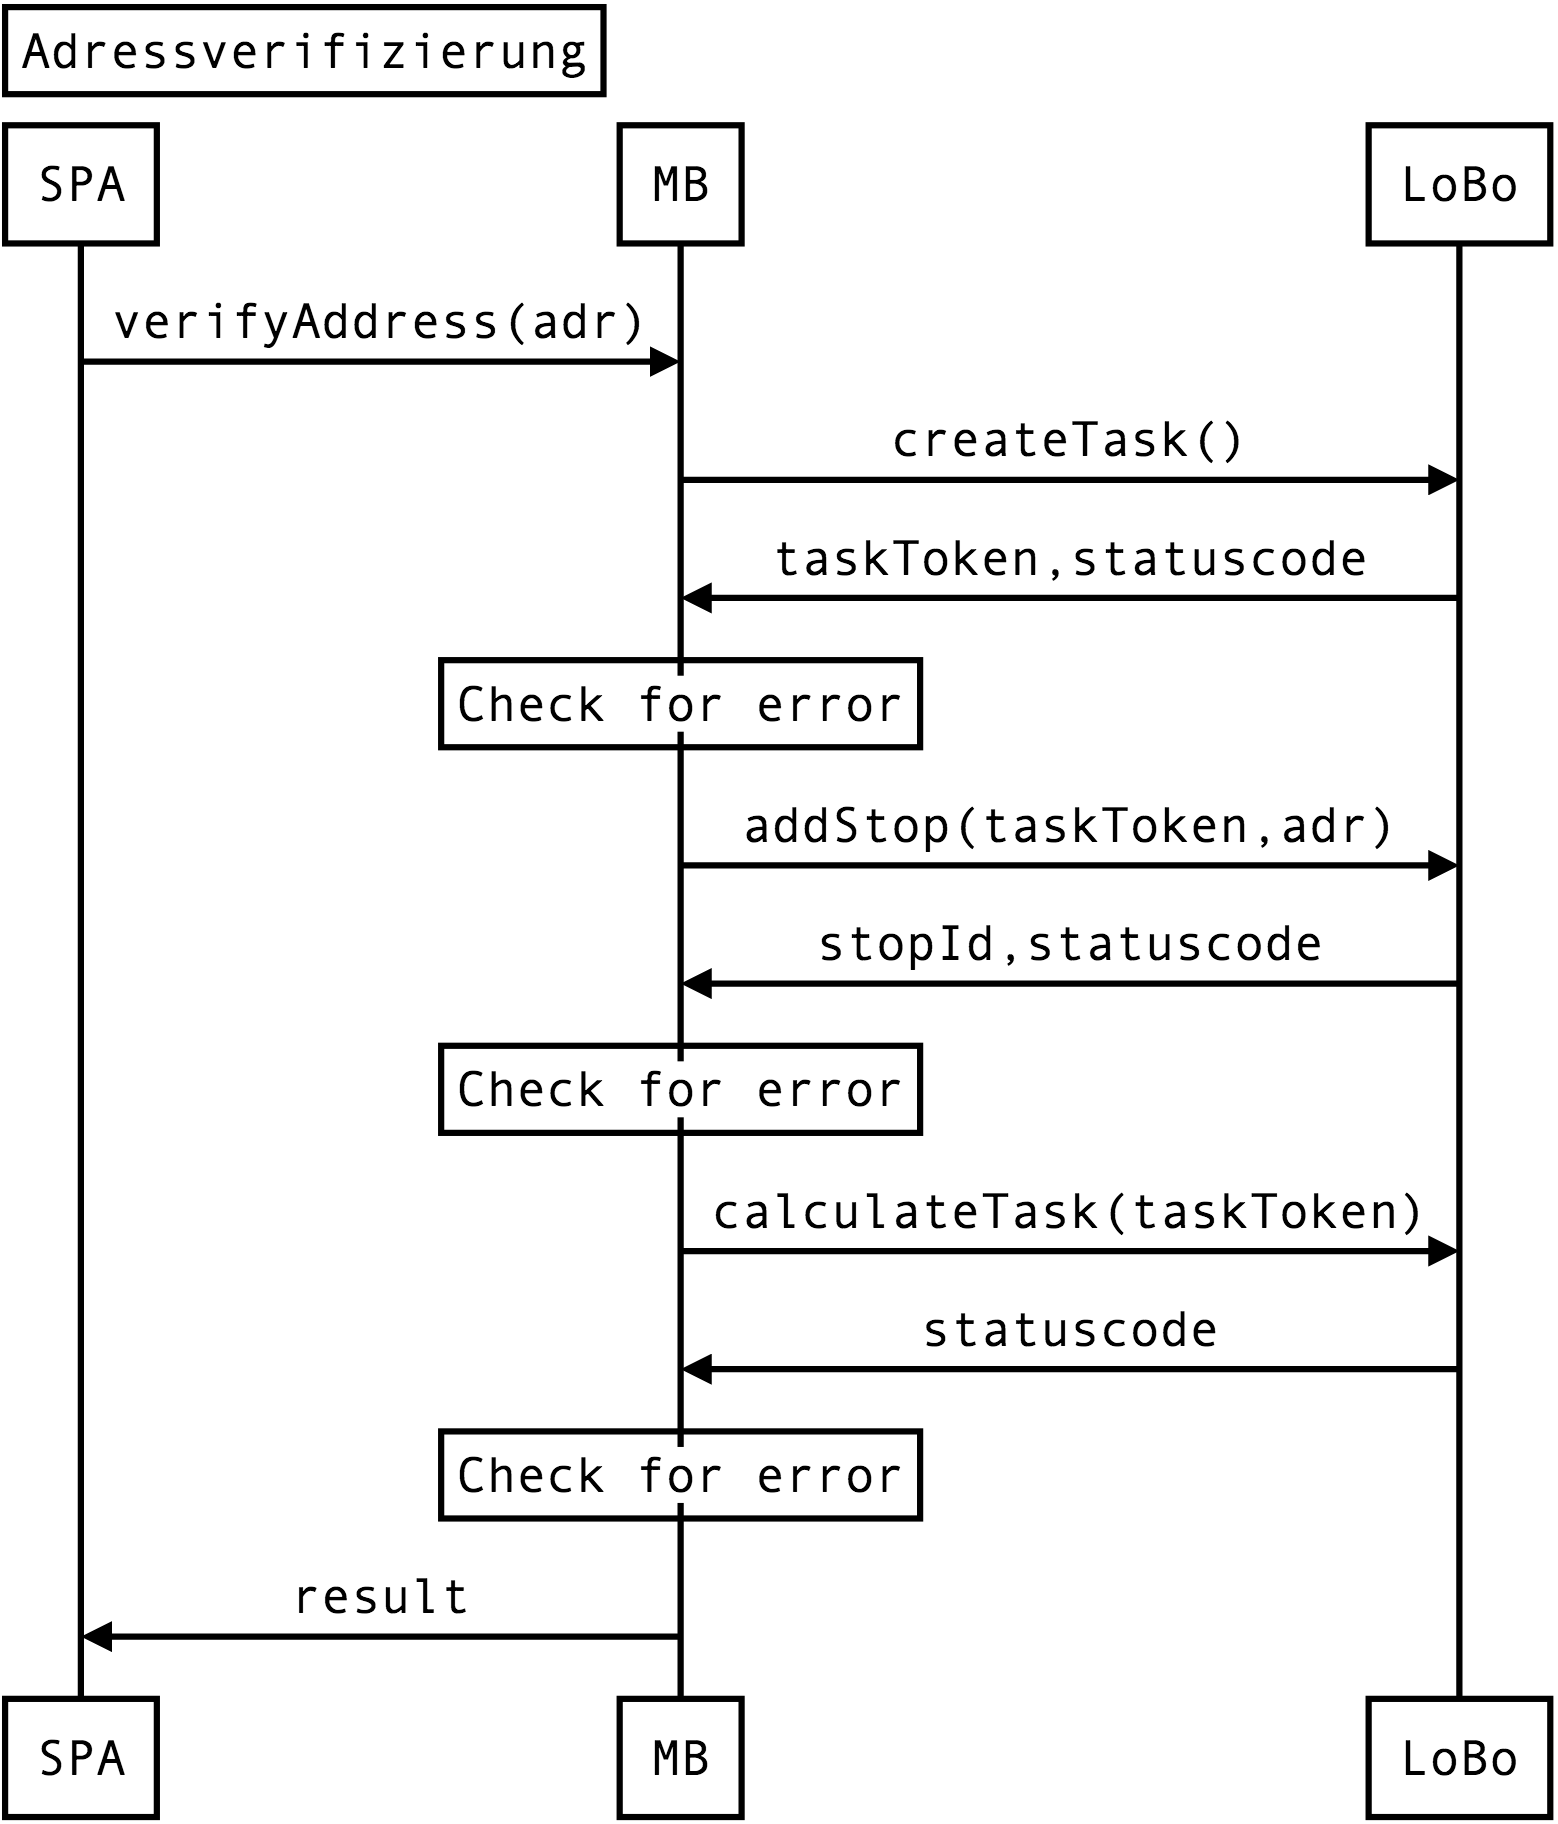
\includegraphics[width=0.88\textwidth]{images/addressverify.png}
	\caption{Darstellung des Prozesses zur Verifizierung einer Adresse}
	\label{fig:addressverify}
\end{figure}

Somit braucht das Mini-Backend nur die Schnittstellenendpunkte zur Verfügung zu stellen, welche auch zwingend von der SPA gebraucht werden. Diese Schnittstellenendpunkte sind in der folgende Liste aufgeführt und beschrieben.

\begin{description}
	\item[createtask] erstellt in Lobo einen neuen Auftrag und übergibt den \textit{tasktoken} an die SPA für alle weiteren anfragen.
	\item[verifyaddress] überprüft in einem temporären Auftrag ob die Adresse im Versorgungsgebiet liegt
	\item[addstop] fügt dem Auftrag eine Adresse hinzu.
	\item[compiletask] überprüft ob dem Auftrag noch weitere Stops (z.B. Bahnhöfe) hinzugefügt werden müssen-
	\item[updatestopinfo] fügt Informationen (z.B. Kontaktpersonen) den einzelnen Adressen hinzu.
	\item[updatestoptime] fügt die Abfahrts- und Ankunftszeit den Stops hinzu.
	\item[updatereftime] erneuert die Uhrzeit wann der Auftrag gestartet wird.
	\item[connections] lädt alle Verbindungen zwischen 2 Städten um eine gewisse Uhrzeit.
	\item[ordertask] finalisiert den Auftrag.
\end{description}

Zusätzlich soll das Mini-Backend soviel Fehler handhaben wie möglich. Die SPA soll Fehler nur bekommen wenn ein Dienst nicht verfügbar ist oder ein schwerwiegender Fehler passiert ist.

\subsection{SPA}
Die primäre Aufgabe der Single-page Applikation ist das Aufnehmen der richtigen Benutzerinformationen und Wiedergeben der daraus berechneten Daten. Die SPA wird in Komponenten aufgeteilt, die einzelne Arbeitsschritte ausführen. Diese Komponenten werden in sogenannten \textit{Step-}Komponenten zusammengefasst. In der Abbildung \ref{fig:comparch} sind die Komponenten und ihre Verwendung grafisch dargestellt. In den folgenden Kapiteln werden die Funktionen der Komponenten beschrieben.

\begin{figure}[ht]
	\centering
  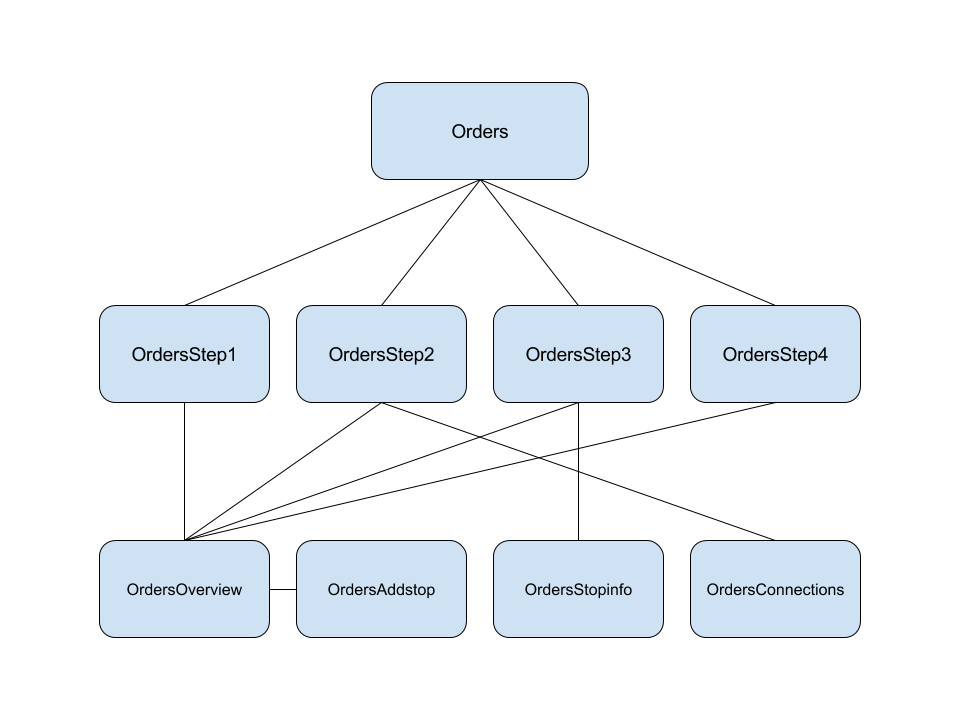
\includegraphics[width=0.88\textwidth]{images/comparch.png}
	\caption{Darstellung der Komponenten und ihrer Verwendung}
	\label{fig:comparch}
\end{figure}

\subsubsection{Orders}
Die Orders Komponente hat keine visuelle Repräsentation. Je nach URL-Pfad wird eine der vier OrdersStep Komponente dargestellt. Die Orders Komponente hat die Aufgabe einen Auftrag zu erstellen und den \textit{tasktoken} zu speichern. Beim  Neuladen der Webseite, ist die Orders Komponente dafür verantwortlich, den letzten Auftrag wieder Aufzunehmen und den entsprechenden Schritt zu laden.

\subsubsection{OrdersOverview}
Die OrdersOverview Komponente wird in jedem Schritt verwendet und zeigt alle relevanten Informationen wie Startzeit, Start- und Zieladresse sowie den Preis des Auftrags. Zusätzlich verwendet die Komponente eine weitere Komponente, welche zur Eingabe der Adressen eingesetzt wird.

\subsubsection{OrdersAddstop}
Die OrdersAddstop Komponente versucht die vom Benutzer eingegebene Adresse zu vervollständigen. Dies geschieht mit der Programmierschnittstelle von Google Maps\footnote{Goole Maps Programmierschnittstelle \url{https://developers.google.com/maps/web}}, welche während der Eingabe des Benutzer versucht, die fertige Adresse anzubieten. Die Komponente verifiziert die Adresse ebenfalls mit LoBo.

\subsubsection{OrdersStopinfo}
Die OrdersStopinfo Komponente bietet dem Benutzer Eingabefelder an, die zur Eingabe für Informationen wie Kontaktperson, Telefonnummer und sonstige Hinweise verwendet werden können.

\subsubsection{OrdersConnections}
Die OrdersConnections Komponente lädt die verfügbaren Bahnverbindungen zwischen zwei Standorten. Die Bahnverbindungen werden mithilfe der Programmierschnittstelle von Opendata.ch\footnote{transport.opendata.ch Programmierschnittstelle \url{https://transport.opendata.ch/}} geladen. Nach erfolgreicher Auswahl des Benutzers werden die Zeitinformationen (Abfahrts- und Ankunftszeit sowie die jeweiligen Bahnsteige) in den jeweiligen Stops in LoBo gespeichert.

\subsubsection{OrdersStep1}
Die OrdersStep1 Komponente ist verantwortlich nach Eingabe der Start und Zieladresse zu übermitteln und den Auftrag zu vervollständigen. Nach erfolgreicher Ausführung wird entweder zur OrdersStep2 oder OrdersStep3 Komponente gewechselt.

\subsubsection{OrdersStep2}
Die OrdersStep2 Komponente ist verantwortlich, die OrdersConnections Komponente darzustellen und nach erfolgreicher Bahnverbindungsauswahl zur OrderStep3 Komponente zu wechseln.

\subsubsection{OrdersStep3}
Die OrdersStep3 Komponente ist verantwortlich, für die jeweiligen Stops (Start und Zeil) die OrdersStopinfo Komponenten anzuzeigen und einen klickbare Aktion, welche den Auftrag vollständig in LoBo einträgt und nach erfolgreicher Durchführung zu der OrdersStep4 Komponente wechselt.

\subsubsection{OrdersStep4}
Die OrdersStep4 Komponente ist verantwortlich, Links zu dem erstellten Bestätigungs PDF sowie zur Auftragsstatus Seite bereit zu stellen.








